In this section, we will explore two types of communication styles and examine how they intervene to manage clock deviation.

\subsection{Communication styles}

\subsubsection{Synchronous communication style}
In synchronous communication, the sender and receiver are synchronized and operate in a lockstep fashion, ensuring that messages are sent and received at \emph{predefined time intervals}. In the example of \fig{fig:conne:synch}, there are two modules: a consumer and a producer. The consumer generates a message, and the producer consumes it upon reception. In this case, synchronization is achieved using the send/receive rule of \fig{fig:prism:rules}.

\noindent
\begin{figure*}[!htb]
    \centering
    


\tikzset{every picture/.style={line width=0.75pt}} %set default line width to 0.75pt        

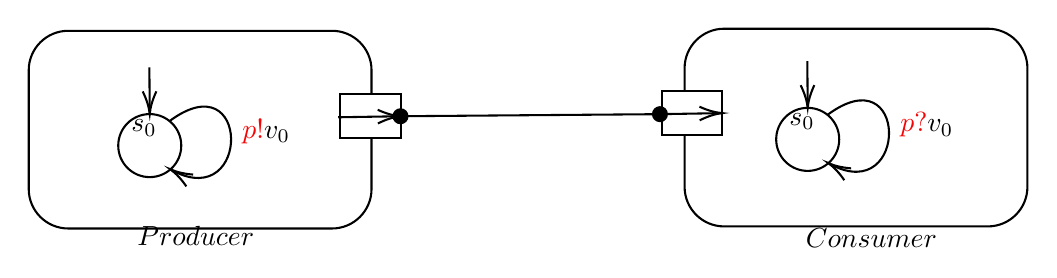
\begin{tikzpicture}[x=0.75pt,y=0.75pt,yscale=-1,xscale=1]
%uncomment if require: \path (0,300); %set diagram left start at 0, and has height of 300

%Rounded Rect [id:dp625014263368401] 
\draw   (48,100.05) .. controls (48,89.53) and (56.53,81) .. (67.05,81) -- (194.12,81) .. controls (204.64,81) and (213.17,89.53) .. (213.17,100.05) -- (213.17,157.2) .. controls (213.17,167.72) and (204.64,176.25) .. (194.12,176.25) -- (67.05,176.25) .. controls (56.53,176.25) and (48,167.72) .. (48,157.2) -- cycle ;
%Rounded Rect [id:dp9966027602076452] 
\draw   (364,99.05) .. controls (364,88.53) and (372.53,80) .. (383.05,80) -- (510.12,80) .. controls (520.64,80) and (529.17,88.53) .. (529.17,99.05) -- (529.17,156.2) .. controls (529.17,166.72) and (520.64,175.25) .. (510.12,175.25) -- (383.05,175.25) .. controls (372.53,175.25) and (364,166.72) .. (364,156.2) -- cycle ;
%Shape: Rectangle [id:dp5720382636417926] 
\draw  [fill={rgb, 255:red, 255; green, 255; blue, 255 }  ,fill opacity=1 ] (198,111.5) -- (227.17,111.5) -- (227.17,132.75) -- (198,132.75) -- cycle ;
%Straight Lines [id:da19839885586208772] 
\draw    (197.13,122.67) -- (225.13,122.2) ;
\draw [shift={(227.13,122.17)}, rotate = 179.05] [color={rgb, 255:red, 0; green, 0; blue, 0 }  ][line width=0.75]    (10.93,-3.29) .. controls (6.95,-1.4) and (3.31,-0.3) .. (0,0) .. controls (3.31,0.3) and (6.95,1.4) .. (10.93,3.29)   ;

%Shape: Circle [id:dp5139718833454837] 
\draw   (91.13,136.31) .. controls (91.13,127.92) and (97.92,121.13) .. (106.31,121.13) .. controls (114.7,121.13) and (121.5,127.92) .. (121.5,136.31) .. controls (121.5,144.7) and (114.7,151.5) .. (106.31,151.5) .. controls (97.92,151.5) and (91.13,144.7) .. (91.13,136.31) -- cycle ;
%Curve Lines [id:da8644908127833736] 
\draw    (115.63,124.67) .. controls (155.03,95.12) and (155.13,167.93) .. (117.85,148.61) ;
\draw [shift={(116.13,147.67)}, rotate = 29.98] [color={rgb, 255:red, 0; green, 0; blue, 0 }  ][line width=0.75]    (10.93,-3.29) .. controls (6.95,-1.4) and (3.31,-0.3) .. (0,0) .. controls (3.31,0.3) and (6.95,1.4) .. (10.93,3.29)   ;
%Straight Lines [id:da9542241932825488] 
\draw    (106.13,98.67) -- (106.3,119.13) ;
\draw [shift={(106.31,121.13)}, rotate = 269.52] [color={rgb, 255:red, 0; green, 0; blue, 0 }  ][line width=0.75]    (10.93,-3.29) .. controls (6.95,-1.4) and (3.31,-0.3) .. (0,0) .. controls (3.31,0.3) and (6.95,1.4) .. (10.93,3.29)   ;

%Shape: Circle [id:dp6922199410406487] 
\draw   (408.13,133.31) .. controls (408.13,124.92) and (414.92,118.13) .. (423.31,118.13) .. controls (431.7,118.13) and (438.5,124.92) .. (438.5,133.31) .. controls (438.5,141.7) and (431.7,148.5) .. (423.31,148.5) .. controls (414.92,148.5) and (408.13,141.7) .. (408.13,133.31) -- cycle ;
%Curve Lines [id:da5423054562376367] 
\draw    (432.63,121.67) .. controls (472.03,92.12) and (472.13,164.93) .. (434.85,145.61) ;
\draw [shift={(433.13,144.67)}, rotate = 29.98] [color={rgb, 255:red, 0; green, 0; blue, 0 }  ][line width=0.75]    (10.93,-3.29) .. controls (6.95,-1.4) and (3.31,-0.3) .. (0,0) .. controls (3.31,0.3) and (6.95,1.4) .. (10.93,3.29)   ;
%Straight Lines [id:da5451612329047202] 
\draw    (423.13,95.67) -- (423.3,116.13) ;
\draw [shift={(423.31,118.13)}, rotate = 269.52] [color={rgb, 255:red, 0; green, 0; blue, 0 }  ][line width=0.75]    (10.93,-3.29) .. controls (6.95,-1.4) and (3.31,-0.3) .. (0,0) .. controls (3.31,0.3) and (6.95,1.4) .. (10.93,3.29)   ;

%Shape: Rectangle [id:dp5695362074890666] 
\draw  [fill={rgb, 255:red, 255; green, 255; blue, 255 }  ,fill opacity=1 ] (353,110) -- (382.17,110) -- (382.17,131.25) -- (353,131.25) -- cycle ;
%Straight Lines [id:da5287521011958595] 
\draw    (352.13,121.17) -- (380.13,120.7) ;
\draw [shift={(382.13,120.67)}, rotate = 179.05] [color={rgb, 255:red, 0; green, 0; blue, 0 }  ][line width=0.75]    (10.93,-3.29) .. controls (6.95,-1.4) and (3.31,-0.3) .. (0,0) .. controls (3.31,0.3) and (6.95,1.4) .. (10.93,3.29)   ;

%Straight Lines [id:da45865603815333666] 
\draw    (227.13,122.17) -- (352.13,121.17) ;
\draw [shift={(352.13,121.17)}, rotate = 359.54] [color={rgb, 255:red, 0; green, 0; blue, 0 }  ][fill={rgb, 255:red, 0; green, 0; blue, 0 }  ][line width=0.75]      (0, 0) circle [x radius= 3.35, y radius= 3.35]   ;
\draw [shift={(227.13,122.17)}, rotate = 359.54] [color={rgb, 255:red, 0; green, 0; blue, 0 }  ][fill={rgb, 255:red, 0; green, 0; blue, 0 }  ][line width=0.75]      (0, 0) circle [x radius= 3.35, y radius= 3.35]   ;


% Text Node
\draw (420.88,175) node [anchor=north west][inner sep=0.75pt]    {$Consumer$};
% Text Node
\draw (98.88,173.5) node [anchor=north west][inner sep=0.75pt]    {$Producer$};
% Text Node
\draw (466.5,119) node [anchor=north west][inner sep=0.75pt]    {$\textcolor[rgb]{0.96,0.02,0.02}{p?} v_{0}$};
% Text Node
\draw (413,119.5) node [anchor=north west][inner sep=0.75pt]    {$s_{0}$};
% Text Node
\draw (149.5,122) node [anchor=north west][inner sep=0.75pt]    {$\textcolor[rgb]{0.96,0.02,0.02}{p!} v_{0}$};
% Text Node
\draw (96,122.5) node [anchor=north west][inner sep=0.75pt]    {$s_{0}$};


\end{tikzpicture}

    \caption{Synchronous Model.}
    \label{fig:conne:synch}
\end{figure*} 


 
\subsubsection{Asynchronous communication style}
Asynchronous communication refers to a communication mechanism where the sender and receiver operate independently of each other. In this type of communication, there is no strict timing or coordination between the sender and receiver. Instead, messages are sent and received asynchronously, allowing each component to operate at its own pace. In the example shown in \fig{fig:conne:asynch}, there are two modules: a consumer and a producer. The consumer generates a message and pushes it to a FIFO buffer, which is managed by another module. When the buffer is full, it is consumed by the consumer module.

\noindent
\begin{figure*}[!htb]
    \centering
    


\tikzset{every picture/.style={line width=0.75pt}} %set default line width to 0.75pt        

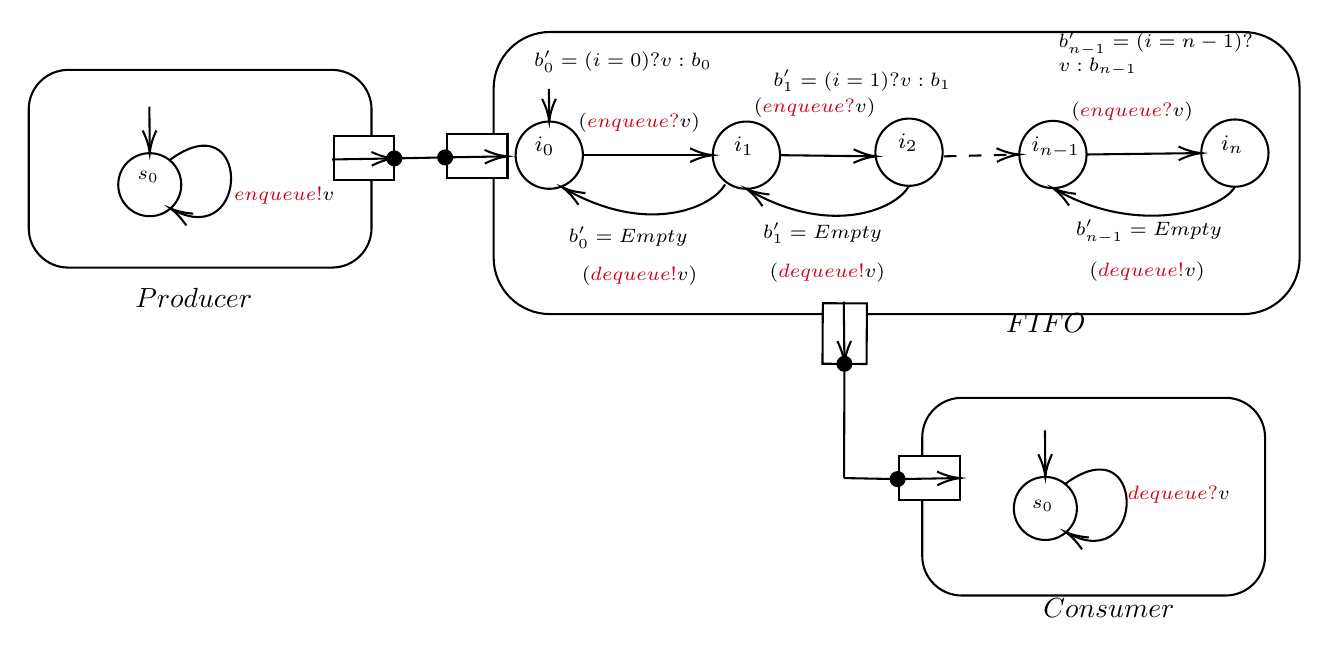
\begin{tikzpicture}[x=0.75pt,y=0.75pt,yscale=-1,xscale=1]
%uncomment if require: \path (0,300); %set diagram left start at 0, and has height of 300

%Rounded Rect [id:dp5077886957226575] 
\draw   (22,42.05) .. controls (22,31.53) and (30.53,23) .. (41.05,23) -- (168.12,23) .. controls (178.64,23) and (187.17,31.53) .. (187.17,42.05) -- (187.17,99.2) .. controls (187.17,109.72) and (178.64,118.25) .. (168.12,118.25) -- (41.05,118.25) .. controls (30.53,118.25) and (22,109.72) .. (22,99.2) -- cycle ;
%Rounded Rect [id:dp6796963511871013] 
\draw   (452.5,200.05) .. controls (452.5,189.53) and (461.03,181) .. (471.55,181) -- (598.62,181) .. controls (609.14,181) and (617.67,189.53) .. (617.67,200.05) -- (617.67,257.2) .. controls (617.67,267.72) and (609.14,276.25) .. (598.62,276.25) -- (471.55,276.25) .. controls (461.03,276.25) and (452.5,267.72) .. (452.5,257.2) -- cycle ;
%Shape: Circle [id:dp48954526237555984] 
\draw   (496.63,234.31) .. controls (496.63,225.92) and (503.42,219.13) .. (511.81,219.13) .. controls (520.2,219.13) and (527,225.92) .. (527,234.31) .. controls (527,242.7) and (520.2,249.5) .. (511.81,249.5) .. controls (503.42,249.5) and (496.63,242.7) .. (496.63,234.31) -- cycle ;
%Curve Lines [id:da5644645023606785] 
\draw    (521.13,222.67) .. controls (560.53,193.12) and (560.63,265.93) .. (523.35,246.61) ;
\draw [shift={(521.63,245.67)}, rotate = 29.98] [color={rgb, 255:red, 0; green, 0; blue, 0 }  ][line width=0.75]    (10.93,-3.29) .. controls (6.95,-1.4) and (3.31,-0.3) .. (0,0) .. controls (3.31,0.3) and (6.95,1.4) .. (10.93,3.29)   ;
%Straight Lines [id:da6370283538427413] 
\draw    (511.63,196.67) -- (511.8,217.13) ;
\draw [shift={(511.81,219.13)}, rotate = 269.52] [color={rgb, 255:red, 0; green, 0; blue, 0 }  ][line width=0.75]    (10.93,-3.29) .. controls (6.95,-1.4) and (3.31,-0.3) .. (0,0) .. controls (3.31,0.3) and (6.95,1.4) .. (10.93,3.29)   ;
%Shape: Rectangle [id:dp7721693985914683] 
\draw  [fill={rgb, 255:red, 255; green, 255; blue, 255 }  ,fill opacity=1 ] (441.5,209) -- (470.67,209) -- (470.67,230.25) -- (441.5,230.25) -- cycle ;
%Straight Lines [id:da714075762069312] 
\draw    (440.63,220.17) -- (468.63,219.7) ;
\draw [shift={(470.63,219.67)}, rotate = 179.05] [color={rgb, 255:red, 0; green, 0; blue, 0 }  ][line width=0.75]    (10.93,-3.29) .. controls (6.95,-1.4) and (3.31,-0.3) .. (0,0) .. controls (3.31,0.3) and (6.95,1.4) .. (10.93,3.29)   ;

%Shape: Rectangle [id:dp9998980436030002] 
\draw  [fill={rgb, 255:red, 255; green, 255; blue, 255 }  ,fill opacity=1 ] (169,55) -- (198.17,55) -- (198.17,76.25) -- (169,76.25) -- cycle ;
%Straight Lines [id:da8143405773569469] 
\draw    (168.13,66.17) -- (196.13,65.7) ;
\draw [shift={(198.13,65.67)}, rotate = 179.05] [color={rgb, 255:red, 0; green, 0; blue, 0 }  ][line width=0.75]    (10.93,-3.29) .. controls (6.95,-1.4) and (3.31,-0.3) .. (0,0) .. controls (3.31,0.3) and (6.95,1.4) .. (10.93,3.29)   ;

%Shape: Circle [id:dp17619550340121215] 
\draw   (65.13,78.31) .. controls (65.13,69.92) and (71.92,63.13) .. (80.31,63.13) .. controls (88.7,63.13) and (95.5,69.92) .. (95.5,78.31) .. controls (95.5,86.7) and (88.7,93.5) .. (80.31,93.5) .. controls (71.92,93.5) and (65.13,86.7) .. (65.13,78.31) -- cycle ;
%Curve Lines [id:da7208507788667503] 
\draw    (89.63,66.67) .. controls (129.03,37.12) and (129.13,109.93) .. (91.85,90.61) ;
\draw [shift={(90.13,89.67)}, rotate = 29.98] [color={rgb, 255:red, 0; green, 0; blue, 0 }  ][line width=0.75]    (10.93,-3.29) .. controls (6.95,-1.4) and (3.31,-0.3) .. (0,0) .. controls (3.31,0.3) and (6.95,1.4) .. (10.93,3.29)   ;
%Straight Lines [id:da5550817830099761] 
\draw    (80.13,40.67) -- (80.3,61.13) ;
\draw [shift={(80.31,63.13)}, rotate = 269.52] [color={rgb, 255:red, 0; green, 0; blue, 0 }  ][line width=0.75]    (10.93,-3.29) .. controls (6.95,-1.4) and (3.31,-0.3) .. (0,0) .. controls (3.31,0.3) and (6.95,1.4) .. (10.93,3.29)   ;
%Shape: Circle [id:dp18366231037577307] 
\draw   (256.6,64.1) .. controls (256.6,55.15) and (263.85,47.9) .. (272.8,47.9) .. controls (281.75,47.9) and (289,55.15) .. (289,64.1) .. controls (289,73.05) and (281.75,80.3) .. (272.8,80.3) .. controls (263.85,80.3) and (256.6,73.05) .. (256.6,64.1) -- cycle ;
%Straight Lines [id:da15359166996791118] 
\draw    (272.6,32.13) -- (272.78,45.9) ;
\draw [shift={(272.8,47.9)}, rotate = 269.29] [color={rgb, 255:red, 0; green, 0; blue, 0 }  ][line width=0.75]    (10.93,-3.29) .. controls (6.95,-1.4) and (3.31,-0.3) .. (0,0) .. controls (3.31,0.3) and (6.95,1.4) .. (10.93,3.29)   ;
%Shape: Circle [id:dp09174175554217379] 
\draw   (351.6,64.1) .. controls (351.6,55.15) and (358.85,47.9) .. (367.8,47.9) .. controls (376.75,47.9) and (384,55.15) .. (384,64.1) .. controls (384,73.05) and (376.75,80.3) .. (367.8,80.3) .. controls (358.85,80.3) and (351.6,73.05) .. (351.6,64.1) -- cycle ;
%Shape: Circle [id:dp7472050147349211] 
\draw   (499.27,63.77) .. controls (499.27,54.82) and (506.52,47.57) .. (515.47,47.57) .. controls (524.41,47.57) and (531.67,54.82) .. (531.67,63.77) .. controls (531.67,72.71) and (524.41,79.97) .. (515.47,79.97) .. controls (506.52,79.97) and (499.27,72.71) .. (499.27,63.77) -- cycle ;
%Straight Lines [id:da5414573338678649] 
\draw    (289,64.1) -- (349.6,64.1) ;
\draw [shift={(351.6,64.1)}, rotate = 180] [color={rgb, 255:red, 0; green, 0; blue, 0 }  ][line width=0.75]    (10.93,-3.29) .. controls (6.95,-1.4) and (3.31,-0.3) .. (0,0) .. controls (3.31,0.3) and (6.95,1.4) .. (10.93,3.29)   ;
%Straight Lines [id:da7528239561309613] 
\draw  [dash pattern={on 4.5pt off 4.5pt}]  (463,64.67) -- (497.27,63.82) ;
\draw [shift={(499.27,63.77)}, rotate = 178.58] [color={rgb, 255:red, 0; green, 0; blue, 0 }  ][line width=0.75]    (10.93,-3.29) .. controls (6.95,-1.4) and (3.31,-0.3) .. (0,0) .. controls (3.31,0.3) and (6.95,1.4) .. (10.93,3.29)   ;
%Shape: Circle [id:dp39040359873777464] 
\draw   (429.93,62.67) .. controls (429.93,53.72) and (437.19,46.47) .. (446.13,46.47) .. controls (455.08,46.47) and (462.33,53.72) .. (462.33,62.67) .. controls (462.33,71.61) and (455.08,78.87) .. (446.13,78.87) .. controls (437.19,78.87) and (429.93,71.61) .. (429.93,62.67) -- cycle ;
%Straight Lines [id:da8273177497883976] 
\draw    (384,64.1) -- (428.33,64.64) ;
\draw [shift={(430.33,64.67)}, rotate = 180.7] [color={rgb, 255:red, 0; green, 0; blue, 0 }  ][line width=0.75]    (10.93,-3.29) .. controls (6.95,-1.4) and (3.31,-0.3) .. (0,0) .. controls (3.31,0.3) and (6.95,1.4) .. (10.93,3.29)   ;
%Shape: Circle [id:dp18603360770873567] 
\draw   (586.93,63.1) .. controls (586.93,54.15) and (594.19,46.9) .. (603.13,46.9) .. controls (612.08,46.9) and (619.33,54.15) .. (619.33,63.1) .. controls (619.33,72.05) and (612.08,79.3) .. (603.13,79.3) .. controls (594.19,79.3) and (586.93,72.05) .. (586.93,63.1) -- cycle ;
%Straight Lines [id:da19534083004381908] 
\draw    (531.67,63.77) -- (584.93,63.12) ;
\draw [shift={(586.93,63.1)}, rotate = 179.31] [color={rgb, 255:red, 0; green, 0; blue, 0 }  ][line width=0.75]    (10.93,-3.29) .. controls (6.95,-1.4) and (3.31,-0.3) .. (0,0) .. controls (3.31,0.3) and (6.95,1.4) .. (10.93,3.29)   ;
%Curve Lines [id:da11236664094083326] 
\draw    (603.13,79.3) .. controls (597.06,90.55) and (556.49,103.41) .. (516.67,80.67) ;
\draw [shift={(515.47,79.97)}, rotate = 30.52] [color={rgb, 255:red, 0; green, 0; blue, 0 }  ][line width=0.75]    (10.93,-3.29) .. controls (6.95,-1.4) and (3.31,-0.3) .. (0,0) .. controls (3.31,0.3) and (6.95,1.4) .. (10.93,3.29)   ;
%Curve Lines [id:da31891726846280266] 
\draw    (446.13,78.87) .. controls (440.06,90.12) and (408.64,103.72) .. (369,81) ;
\draw [shift={(367.8,80.3)}, rotate = 30.52] [color={rgb, 255:red, 0; green, 0; blue, 0 }  ][line width=0.75]    (10.93,-3.29) .. controls (6.95,-1.4) and (3.31,-0.3) .. (0,0) .. controls (3.31,0.3) and (6.95,1.4) .. (10.93,3.29)   ;
%Curve Lines [id:da16869767907947275] 
\draw    (357.47,78.2) .. controls (351.39,89.45) and (319.97,103.06) .. (280.34,80.33) ;
\draw [shift={(279.13,79.63)}, rotate = 30.52] [color={rgb, 255:red, 0; green, 0; blue, 0 }  ][line width=0.75]    (10.93,-3.29) .. controls (6.95,-1.4) and (3.31,-0.3) .. (0,0) .. controls (3.31,0.3) and (6.95,1.4) .. (10.93,3.29)   ;
%Rounded Rect [id:dp8051559743906143] 
\draw   (246,31.93) .. controls (246,16.92) and (258.17,4.75) .. (273.18,4.75) -- (607.15,4.75) .. controls (622.16,4.75) and (634.33,16.92) .. (634.33,31.93) -- (634.33,113.48) .. controls (634.33,128.5) and (622.16,140.67) .. (607.15,140.67) -- (273.18,140.67) .. controls (258.17,140.67) and (246,128.5) .. (246,113.48) -- cycle ;
%Shape: Rectangle [id:dp7329790049933834] 
\draw  [fill={rgb, 255:red, 255; green, 255; blue, 255 }  ,fill opacity=1 ] (223.5,54) -- (252.67,54) -- (252.67,75.25) -- (223.5,75.25) -- cycle ;
%Straight Lines [id:da35031986622531375] 
\draw    (222.63,65.17) -- (250.63,64.7) ;
\draw [shift={(252.63,64.67)}, rotate = 179.05] [color={rgb, 255:red, 0; green, 0; blue, 0 }  ][line width=0.75]    (10.93,-3.29) .. controls (6.95,-1.4) and (3.31,-0.3) .. (0,0) .. controls (3.31,0.3) and (6.95,1.4) .. (10.93,3.29)   ;

%Shape: Rectangle [id:dp05043429256580323] 
\draw  [fill={rgb, 255:red, 255; green, 255; blue, 255 }  ,fill opacity=1 ] (425.85,135.54) -- (425.68,164.71) -- (404.43,164.58) -- (404.6,135.42) -- cycle ;
%Straight Lines [id:da977653573737004] 
\draw    (414.69,134.6) -- (414.99,162.6) ;
\draw [shift={(415.02,164.6)}, rotate = 269.39] [color={rgb, 255:red, 0; green, 0; blue, 0 }  ][line width=0.75]    (10.93,-3.29) .. controls (6.95,-1.4) and (3.31,-0.3) .. (0,0) .. controls (3.31,0.3) and (6.95,1.4) .. (10.93,3.29)   ;

%Straight Lines [id:da6228866579240351] 
\draw    (198.13,65.67) -- (222.63,65.17) ;
\draw [shift={(222.63,65.17)}, rotate = 358.83] [color={rgb, 255:red, 0; green, 0; blue, 0 }  ][fill={rgb, 255:red, 0; green, 0; blue, 0 }  ][line width=0.75]      (0, 0) circle [x radius= 3.35, y radius= 3.35]   ;
\draw [shift={(198.13,65.67)}, rotate = 358.83] [color={rgb, 255:red, 0; green, 0; blue, 0 }  ][fill={rgb, 255:red, 0; green, 0; blue, 0 }  ][line width=0.75]      (0, 0) circle [x radius= 3.35, y radius= 3.35]   ;
%Straight Lines [id:da07540077874823459] 
\draw    (415.02,164.6) -- (414.83,219.67) ;
\draw [shift={(415.02,164.6)}, rotate = 90.19] [color={rgb, 255:red, 0; green, 0; blue, 0 }  ][fill={rgb, 255:red, 0; green, 0; blue, 0 }  ][line width=0.75]      (0, 0) circle [x radius= 3.35, y radius= 3.35]   ;
%Straight Lines [id:da4496253599648107] 
\draw    (440.63,220.17) -- (414.83,219.67) ;
\draw [shift={(440.63,220.17)}, rotate = 181.11] [color={rgb, 255:red, 0; green, 0; blue, 0 }  ][fill={rgb, 255:red, 0; green, 0; blue, 0 }  ][line width=0.75]      (0, 0) circle [x radius= 3.35, y radius= 3.35]   ;


% Text Node
\draw (491.38,139) node [anchor=north west][inner sep=0.75pt]    {$FIFO$};
% Text Node
\draw (531.5,114) node [anchor=north west][inner sep=0.75pt]  [font=\scriptsize]  {$(\textcolor[rgb]{0.82,0.01,0.11}{dequeue!} v)$};
% Text Node
\draw (377.5,114.5) node [anchor=north west][inner sep=0.75pt]  [font=\scriptsize]  {$(\textcolor[rgb]{0.82,0.01,0.11}{dequeue!} v)$};
% Text Node
\draw (522.83,37.17) node [anchor=north west][inner sep=0.75pt]  [font=\scriptsize]  {$(\textcolor[rgb]{0.82,0.01,0.11}{enqueue?} v)$};
% Text Node
\draw (369.83,35.17) node [anchor=north west][inner sep=0.75pt]  [font=\scriptsize]  {$(\textcolor[rgb]{0.82,0.01,0.11}{enqueue?} v)$};
% Text Node
\draw (550,222) node [anchor=north west][inner sep=0.75pt]  [font=\scriptsize]  {$\textcolor[rgb]{0.82,0.01,0.11}{dequeue?} v$};
% Text Node
\draw (504,229) node [anchor=north west][inner sep=0.75pt]  [font=\scriptsize]  {$s_{0}$};
% Text Node
\draw (509.38,276) node [anchor=north west][inner sep=0.75pt]    {$Consumer$};
% Text Node
\draw (119.5,78) node [anchor=north west][inner sep=0.75pt]  [font=\scriptsize]  {$\textcolor[rgb]{0.82,0.01,0.11}{enqueue!} v$};
% Text Node
\draw (73,70.5) node [anchor=north west][inner sep=0.75pt]  [font=\scriptsize]  {$s_{0}$};
% Text Node
\draw (287,116) node [anchor=north west][inner sep=0.75pt]  [font=\scriptsize]  {$(\textcolor[rgb]{0.82,0.01,0.11}{dequeue!} v)$};
% Text Node
\draw (280.67,97) node [anchor=north west][inner sep=0.75pt]  [font=\scriptsize]  {$b_{0} '=Empty$};
% Text Node
\draw (374.33,95) node [anchor=north west][inner sep=0.75pt]  [font=\scriptsize]  {$b_{1} '=Empty$};
% Text Node
\draw (510,3.17) node [anchor=north west][inner sep=0.75pt]  [font=\scriptsize]  {$ \begin{array}{l}
b_{n-1} '=( i=n-1) ?\\
v:b_{n-1}
\end{array}$};
% Text Node
\draw (595,53.33) node [anchor=north west][inner sep=0.75pt]  [font=\footnotesize]  {$i_{n}$};
% Text Node
\draw (439.33,52.33) node [anchor=north west][inner sep=0.75pt]  [font=\footnotesize]  {$i_{2}$};
% Text Node
\draw (525,93.67) node [anchor=north west][inner sep=0.75pt]  [font=\scriptsize]  {$b_{n-1} '=Empty$};
% Text Node
\draw (379.33,21.67) node [anchor=north west][inner sep=0.75pt]  [font=\scriptsize]  {$b_{1} '=( i=1) ?v:b_{1}$};
% Text Node
\draw (264,12.33) node [anchor=north west][inner sep=0.75pt]  [font=\scriptsize]  {$b_{0} '=( i=0) ?v:b_{0}$};
% Text Node
\draw (285.33,42.17) node [anchor=north west][inner sep=0.75pt]  [font=\scriptsize]  {$(\textcolor[rgb]{0.82,0.01,0.11}{enqueue?} v)$};
% Text Node
\draw (503.67,54) node [anchor=north west][inner sep=0.75pt]  [font=\footnotesize]  {$i_{n-1}$};
% Text Node
\draw (360.33,54) node [anchor=north west][inner sep=0.75pt]  [font=\footnotesize]  {$i_{1}$};
% Text Node
\draw (264.33,54) node [anchor=north west][inner sep=0.75pt]  [font=\footnotesize]  {$i_{0}$};
% Text Node
\draw (71.88,126.5) node [anchor=north west][inner sep=0.75pt]    {$Producer$};


\end{tikzpicture}

    \caption{Asynchronous Model.}
    \label{fig:conne:asynch}
\end{figure*} 


The FIFO module includes buffer variables, namely \emath{b_{0}} and \emath{b_{n}}, as well as an index \emath{i} that is incremented each time new data is received and stored in \emath{b_{i}}. Furthermore, the asynchronous communication style must adhere to the following rules: \ref{Enqueue} and \ref{Dequeue}.


\begin{boxD}
%\framedtext{
	      \begin{equation} \label{Enqueue}\frac{ x_{0} \xrightarrow{g:enqueue!v} {x'_{0}} \wedge \theta_{0} \models g_{0} \wedge x_{1} \xrightarrow{g:enqueue?v} {x'_{1}} \wedge \theta_{1} \models g_{1}} { \langle x_{0},\ldots,x_{i}, \ldots,x_{n},\theta\rangle \xrightarrow{a}\langle x_{0},\ldots,x'_{i}, \ldots,x_{n},\theta'\rangle  } \tag{Enqueue} \end{equation} where \emath{\theta':=\theta[ b_{i}:=v]}
%}
	      \begin{equation}\label{Dequeue}\frac{ x_{2} \xrightarrow{g:dequeue!v{x'_{2}}} \wedge \theta_{2} \models g_{2} \wedge x_{3} \xrightarrow{g:dequeue?v} {x'_{3}} \wedge \theta_{3} \models g_{3} } { \langle x_{0},\ldots,x_{i}, \ldots,x_{n},\theta\rangle \xrightarrow{a}_{\lambda}\langle x_{0},\ldots,x'_{i}, \ldots,x_{n},\theta'\rangle  } \tag{Dequeue} \end{equation} where \emath{\theta':=\theta[ v:=b_{i}]}
\end{boxD}

\subsection{Clock deviation and mitigation}
\subsubsection{Clock deviation}
In the absence of synchronization, device clocks operate autonomously without coordination. Each component sends its data at its own clock frequency without acknowledgment of a reference clock. Considering \fig{fig:conne:drift}, the device propagates its data at the clock instant \emath{t_{c}+1} with probability \emath{\lambda_{1}} or the device propagates the data at the clock instant \emath{t_{c} + t_{drift}} with probability \emath{\lambda_{2}}, where \emath{t_{drift}} represents the additional elapsed time since the last propagation of internal data by the device. The corresponding rule for clock drifting is portrayed by the rule \ref{unsynch}.

\noindent
\begin{figure*}[!htb]
    \centering
    


\tikzset{every picture/.style={line width=0.75pt}} %set default line width to 0.75pt        

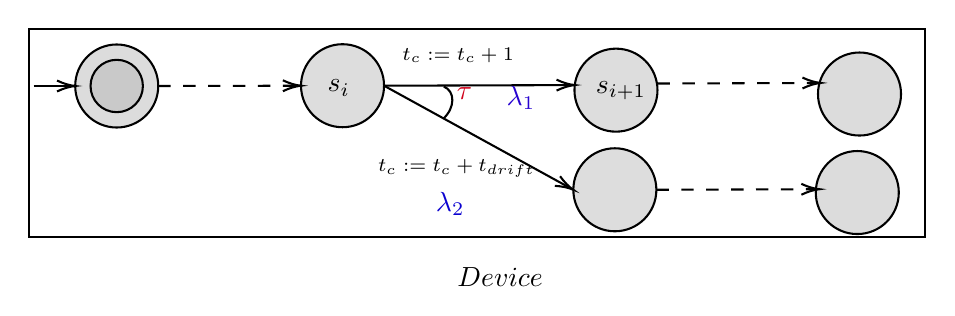
\begin{tikzpicture}[x=0.60pt,y=0.60pt,yscale=-1,xscale=1]
%uncomment if require: \path (0,300); %set diagram left start at 0, and has height of 300

%Shape: Circle [id:dp0800372807837828] 
\draw  [fill={rgb, 255:red, 155; green, 155; blue, 155 }  ,fill opacity=0.34 ] (193.33,42.5) .. controls (193.33,28.69) and (204.53,17.5) .. (218.33,17.5) .. controls (232.14,17.5) and (243.33,28.69) .. (243.33,42.5) .. controls (243.33,56.31) and (232.14,67.5) .. (218.33,67.5) .. controls (204.53,67.5) and (193.33,56.31) .. (193.33,42.5) -- cycle ;
%Shape: Circle [id:dp6517135602121005] 
\draw  [fill={rgb, 255:red, 155; green, 155; blue, 155 }  ,fill opacity=0.34 ] (358,45.17) .. controls (358,31.36) and (369.19,20.17) .. (383,20.17) .. controls (396.81,20.17) and (408,31.36) .. (408,45.17) .. controls (408,58.97) and (396.81,70.17) .. (383,70.17) .. controls (369.19,70.17) and (358,58.97) .. (358,45.17) -- cycle ;
%Shape: Circle [id:dp020288374699267364] 
\draw  [fill={rgb, 255:red, 155; green, 155; blue, 155 }  ,fill opacity=0.35 ] (504.67,47.5) .. controls (504.67,33.69) and (515.86,22.5) .. (529.67,22.5) .. controls (543.47,22.5) and (554.67,33.69) .. (554.67,47.5) .. controls (554.67,61.31) and (543.47,72.5) .. (529.67,72.5) .. controls (515.86,72.5) and (504.67,61.31) .. (504.67,47.5) -- cycle ;
%Shape: Circle [id:dp8120002198294831] 
\draw  [fill={rgb, 255:red, 155; green, 155; blue, 155 }  ,fill opacity=0.35 ] (57.33,42.67) .. controls (57.33,28.86) and (68.53,17.67) .. (82.33,17.67) .. controls (96.14,17.67) and (107.33,28.86) .. (107.33,42.67) .. controls (107.33,56.47) and (96.14,67.67) .. (82.33,67.67) .. controls (68.53,67.67) and (57.33,56.47) .. (57.33,42.67) -- cycle ;
%Straight Lines [id:da06780717013530502] 
\draw  [dash pattern={on 4.5pt off 4.5pt}]  (107.33,42.67) -- (191.33,42.5) ;
\draw [shift={(193.33,42.5)}, rotate = 179.89] [color={rgb, 255:red, 0; green, 0; blue, 0 }  ][line width=0.75]    (10.93,-3.29) .. controls (6.95,-1.4) and (3.31,-0.3) .. (0,0) .. controls (3.31,0.3) and (6.95,1.4) .. (10.93,3.29)   ;
%Straight Lines [id:da8484939119584262] 
\draw    (243.33,42.5) -- (356.15,42.12) ;
\draw [shift={(358.15,42.11)}, rotate = 179.81] [color={rgb, 255:red, 0; green, 0; blue, 0 }  ][line width=0.75]    (10.93,-3.29) .. controls (6.95,-1.4) and (3.31,-0.3) .. (0,0) .. controls (3.31,0.3) and (6.95,1.4) .. (10.93,3.29)   ;
%Straight Lines [id:da5499753499142862] 
\draw  [dash pattern={on 4.5pt off 4.5pt}]  (408,41.17) -- (504.25,40.84) ;
\draw [shift={(506.25,40.83)}, rotate = 179.81] [color={rgb, 255:red, 0; green, 0; blue, 0 }  ][line width=0.75]    (10.93,-3.29) .. controls (6.95,-1.4) and (3.31,-0.3) .. (0,0) .. controls (3.31,0.3) and (6.95,1.4) .. (10.93,3.29)   ;
%Straight Lines [id:da8750765790283018] 
\draw    (32.33,42.67) -- (55.33,42.67) ;
\draw [shift={(57.33,42.67)}, rotate = 180] [color={rgb, 255:red, 0; green, 0; blue, 0 }  ][line width=0.75]    (10.93,-3.29) .. controls (6.95,-1.4) and (3.31,-0.3) .. (0,0) .. controls (3.31,0.3) and (6.95,1.4) .. (10.93,3.29)   ;
%Shape: Circle [id:dp9577830715523987] 
\draw  [fill={rgb, 255:red, 155; green, 155; blue, 155 }  ,fill opacity=0.29 ] (66.56,42.67) .. controls (66.56,33.96) and (73.62,26.9) .. (82.33,26.9) .. controls (91.04,26.9) and (98.1,33.96) .. (98.1,42.67) .. controls (98.1,51.38) and (91.04,58.44) .. (82.33,58.44) .. controls (73.62,58.44) and (66.56,51.38) .. (66.56,42.67) -- cycle ;
%Shape: Rectangle [id:dp759633067613265] 
\draw   (29.33,8.17) -- (569.29,8.17) -- (569.29,133.8) -- (29.33,133.8) -- cycle ;
%Shape: Circle [id:dp5232490962749833] 
\draw  [fill={rgb, 255:red, 155; green, 155; blue, 155 }  ,fill opacity=0.34 ] (357.33,105.17) .. controls (357.33,91.36) and (368.53,80.17) .. (382.33,80.17) .. controls (396.14,80.17) and (407.33,91.36) .. (407.33,105.17) .. controls (407.33,118.97) and (396.14,130.17) .. (382.33,130.17) .. controls (368.53,130.17) and (357.33,118.97) .. (357.33,105.17) -- cycle ;
%Shape: Circle [id:dp6752098325857876] 
\draw  [fill={rgb, 255:red, 155; green, 155; blue, 155 }  ,fill opacity=0.35 ] (503.33,106.83) .. controls (503.33,93.03) and (514.53,81.83) .. (528.33,81.83) .. controls (542.14,81.83) and (553.33,93.03) .. (553.33,106.83) .. controls (553.33,120.64) and (542.14,131.83) .. (528.33,131.83) .. controls (514.53,131.83) and (503.33,120.64) .. (503.33,106.83) -- cycle ;
%Straight Lines [id:da7293836315789196] 
\draw  [dash pattern={on 4.5pt off 4.5pt}]  (407.33,105.17) -- (503.58,104.84) ;
\draw [shift={(505.58,104.83)}, rotate = 179.81] [color={rgb, 255:red, 0; green, 0; blue, 0 }  ][line width=0.75]    (10.93,-3.29) .. controls (6.95,-1.4) and (3.31,-0.3) .. (0,0) .. controls (3.31,0.3) and (6.95,1.4) .. (10.93,3.29)   ;
%Straight Lines [id:da5166679562063851] 
\draw    (243.33,42.5) -- (355.58,104.2) ;
\draw [shift={(357.33,105.17)}, rotate = 208.8] [color={rgb, 255:red, 0; green, 0; blue, 0 }  ][line width=0.75]    (10.93,-3.29) .. controls (6.95,-1.4) and (3.31,-0.3) .. (0,0) .. controls (3.31,0.3) and (6.95,1.4) .. (10.93,3.29)   ;
%Curve Lines [id:da46003188830589814] 
\draw    (279.33,43) .. controls (286.24,45.8) and (286.24,55.8) .. (278.91,62.47) ;


% Text Node
\draw (285.33,42) node [anchor=north west][inner sep=0.75pt]  [color={rgb, 255:red, 208; green, 2; blue, 27 }  ,opacity=1 ]  {$\tau $};
% Text Node
\draw (272.67,104.67) node [anchor=north west][inner sep=0.75pt]  [color={rgb, 255:red, 11; green, 2; blue, 208 }  ,opacity=1 ]  {$\boldsymbol{\lambda _{2}}$};
% Text Node
\draw (315.33,40.67) node [anchor=north west][inner sep=0.75pt]  [color={rgb, 255:red, 39; green, 2; blue, 208 }  ,opacity=1 ]  {$\boldsymbol{\lambda _{1}}$};
% Text Node
\draw (237.83,85.33) node [anchor=north west][inner sep=0.75pt]  [font=\scriptsize,color={rgb, 255:red, 0; green, 0; blue, 0 }  ,opacity=1 ]  {$\boldsymbol{t_{c} :=t_{c} +t_{drift}}$};
% Text Node
\draw (285.67,150) node [anchor=north west][inner sep=0.75pt]    {$Device\ $};
% Text Node
\draw (252.5,17.67) node [anchor=north west][inner sep=0.75pt]  [font=\scriptsize,color={rgb, 255:red, 0; green, 0; blue, 0 }  ,opacity=1 ]  {$\boldsymbol{t_{c} :=t_{c} +1}$};
% Text Node
\draw (369.03,38.17) node [anchor=north west][inner sep=0.75pt]    {$s_{i+1}$};
% Text Node
\draw (207.53,37.17) node [anchor=north west][inner sep=0.75pt]    {$s_{i}$};


\end{tikzpicture}

    \caption{Clock Deviation.}
    \label{fig:conne:drift}
\end{figure*} 
\begin{boxD}
%\framedtext{
	      \begin{equation} \label{unsynch}\frac{ s_{i} \xrightarrow{g:\tau}_{\lambda_{2}} {s'_{i}} \wedge \theta_{0} \models g_{0} } { \langle s_{i}, \ldots,\theta\rangle \xrightarrow{\tau}_{\lambda_{2}}\langle s'_{i}, \ldots\theta'\rangle}   \tag{\emph{Clock drift}} \end{equation} where \emath{\theta':=\theta[ t_{c}:=t_{c}+t_{drift}]}
%}
	      \begin{equation}\label{synch}\frac{ \sset{s_{i} \xrightarrow{g:dequeue!v}s'_{i}} \wedge \sset{s_{j} \xrightarrow{g:dequeue?t_{c}} {s'_{j}}}  \wedge \sset{s_{k} \xrightarrow{g:dequeue?t_{c}} {s'_{k}}} \wedge \theta \models g_{i} \wedge g_{j} \wedge g_{k} } { \langle s_{i},\ldots,s_{j}, \ldots,s_{k},\theta\rangle \xrightarrow{a}_{\lambda}\langle s'_{i},\ldots,s'_{j}, \ldots,s'_{k}, \ldots,\theta'\rangle  } \tag{\emph{Synchronized Clock}} \end{equation} where \emath{\theta':=\theta[ t_{c}:=v]}
\end{boxD}
\subsubsection{Clock deviation mitigation}

Clock drift mitigation consists of specifying an intermediary component or coordinator that resets the internal clock to the average of the clocks received from devices as asserted by \cite{WebsterBDFM18}. In the proposed approach, the coordinator collects all clocks using the FIFO principle, as defined in the asynchronous message passing discussed in the previous subsections (using \emph{enqueue} port to store clocks in variables). Once the clocks are collected, an averaging calculation is performed. Finally, the new clock value is sent back to the devices accordingly, as depicted by the operational semantics rule \ref{synch}. The state variables \emath{s_{i}}, \emath{s_{j}}, and \emath{s_{k}} refer to the FIFO states and devices states, respectively.
 \noindent
\begin{figure*}[!htb]
    \centering
    


\tikzset{every picture/.style={line width=0.75pt}} %set default line width to 0.75pt        

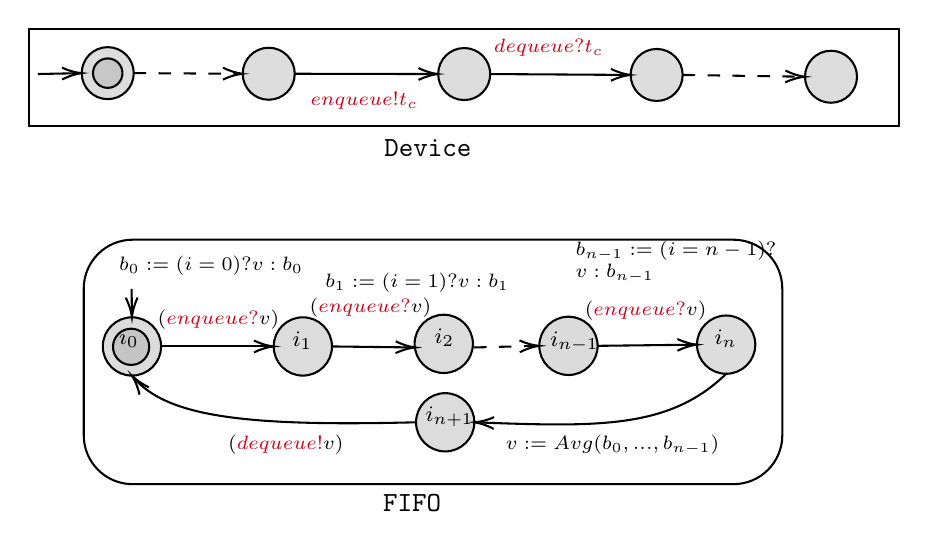
\begin{tikzpicture}[x=0.65pt,y=0.65pt,yscale=-1,xscale=1]
%uncomment if require: \path (0,300); %set diagram left start at 0, and has height of 300

%Shape: Circle [id:dp621785514791322] 
\draw  [fill={rgb, 255:red, 155; green, 155; blue, 155 }  ,fill opacity=0.35 ] (119.43,191.27) .. controls (119.43,182.32) and (126.69,175.07) .. (135.63,175.07) .. controls (144.58,175.07) and (151.83,182.32) .. (151.83,191.27) .. controls (151.83,200.21) and (144.58,207.47) .. (135.63,207.47) .. controls (126.69,207.47) and (119.43,200.21) .. (119.43,191.27) -- cycle ;
%Straight Lines [id:da5710248392373312] 
\draw    (135.44,159.29) -- (135.61,173.07) ;
\draw [shift={(135.63,175.07)}, rotate = 269.29] [color={rgb, 255:red, 0; green, 0; blue, 0 }  ][line width=0.75]    (10.93,-3.29) .. controls (6.95,-1.4) and (3.31,-0.3) .. (0,0) .. controls (3.31,0.3) and (6.95,1.4) .. (10.93,3.29)   ;
%Shape: Circle [id:dp37657262077982245] 
\draw  [fill={rgb, 255:red, 155; green, 155; blue, 155 }  ,fill opacity=0.35 ] (214.43,191.27) .. controls (214.43,182.32) and (221.69,175.07) .. (230.63,175.07) .. controls (239.58,175.07) and (246.83,182.32) .. (246.83,191.27) .. controls (246.83,200.21) and (239.58,207.47) .. (230.63,207.47) .. controls (221.69,207.47) and (214.43,200.21) .. (214.43,191.27) -- cycle ;
%Shape: Circle [id:dp280904277899374] 
\draw  [fill={rgb, 255:red, 155; green, 155; blue, 155 }  ,fill opacity=0.36 ] (362.1,190.93) .. controls (362.1,181.99) and (369.35,174.73) .. (378.3,174.73) .. controls (387.25,174.73) and (394.5,181.99) .. (394.5,190.93) .. controls (394.5,199.88) and (387.25,207.13) .. (378.3,207.13) .. controls (369.35,207.13) and (362.1,199.88) .. (362.1,190.93) -- cycle ;
%Straight Lines [id:da25370273323872616] 
\draw    (151.83,191.27) -- (212.43,191.27) ;
\draw [shift={(214.43,191.27)}, rotate = 180] [color={rgb, 255:red, 0; green, 0; blue, 0 }  ][line width=0.75]    (10.93,-3.29) .. controls (6.95,-1.4) and (3.31,-0.3) .. (0,0) .. controls (3.31,0.3) and (6.95,1.4) .. (10.93,3.29)   ;
%Straight Lines [id:da11175224192841304] 
\draw  [dash pattern={on 4.5pt off 4.5pt}]  (325.83,191.83) -- (360.1,190.98) ;
\draw [shift={(362.1,190.93)}, rotate = 178.58] [color={rgb, 255:red, 0; green, 0; blue, 0 }  ][line width=0.75]    (10.93,-3.29) .. controls (6.95,-1.4) and (3.31,-0.3) .. (0,0) .. controls (3.31,0.3) and (6.95,1.4) .. (10.93,3.29)   ;
%Shape: Circle [id:dp1216688190539813] 
\draw  [fill={rgb, 255:red, 155; green, 155; blue, 155 }  ,fill opacity=0.35 ] (292.77,189.83) .. controls (292.77,180.89) and (300.02,173.63) .. (308.97,173.63) .. controls (317.91,173.63) and (325.17,180.89) .. (325.17,189.83) .. controls (325.17,198.78) and (317.91,206.03) .. (308.97,206.03) .. controls (300.02,206.03) and (292.77,198.78) .. (292.77,189.83) -- cycle ;
%Straight Lines [id:da2654655987954182] 
\draw    (246.83,191.27) -- (291.17,191.81) ;
\draw [shift={(293.17,191.83)}, rotate = 180.7] [color={rgb, 255:red, 0; green, 0; blue, 0 }  ][line width=0.75]    (10.93,-3.29) .. controls (6.95,-1.4) and (3.31,-0.3) .. (0,0) .. controls (3.31,0.3) and (6.95,1.4) .. (10.93,3.29)   ;
%Shape: Circle [id:dp11700483520927796] 
\draw  [fill={rgb, 255:red, 155; green, 155; blue, 155 }  ,fill opacity=0.34 ] (449.77,190.27) .. controls (449.77,181.32) and (457.02,174.07) .. (465.97,174.07) .. controls (474.91,174.07) and (482.17,181.32) .. (482.17,190.27) .. controls (482.17,199.21) and (474.91,206.47) .. (465.97,206.47) .. controls (457.02,206.47) and (449.77,199.21) .. (449.77,190.27) -- cycle ;
%Straight Lines [id:da5609163868748465] 
\draw    (394.5,190.93) -- (447.77,190.29) ;
\draw [shift={(449.77,190.27)}, rotate = 179.31] [color={rgb, 255:red, 0; green, 0; blue, 0 }  ][line width=0.75]    (10.93,-3.29) .. controls (6.95,-1.4) and (3.31,-0.3) .. (0,0) .. controls (3.31,0.3) and (6.95,1.4) .. (10.93,3.29)   ;
%Curve Lines [id:da12392134072596717] 
\draw    (465.97,206.47) .. controls (434.4,237.15) and (395.13,235.99) .. (327,233.47) ;
\draw [shift={(325.97,233.43)}, rotate = 2.12] [color={rgb, 255:red, 0; green, 0; blue, 0 }  ][line width=0.75]    (10.93,-3.29) .. controls (6.95,-1.4) and (3.31,-0.3) .. (0,0) .. controls (3.31,0.3) and (6.95,1.4) .. (10.93,3.29)   ;
%Rounded Rect [id:dp10769156861818274] 
\draw   (108.83,159.1) .. controls (108.83,144.09) and (121,131.92) .. (136.02,131.92) -- (469.98,131.92) .. controls (485,131.92) and (497.17,144.09) .. (497.17,159.1) -- (497.17,240.65) .. controls (497.17,255.66) and (485,267.83) .. (469.98,267.83) -- (136.02,267.83) .. controls (121,267.83) and (108.83,255.66) .. (108.83,240.65) -- cycle ;
%Shape: Circle [id:dp417065956025657] 
\draw  [fill={rgb, 255:red, 155; green, 155; blue, 155 }  ,fill opacity=0.35 ] (293.57,233.43) .. controls (293.57,224.49) and (300.82,217.23) .. (309.77,217.23) .. controls (318.71,217.23) and (325.97,224.49) .. (325.97,233.43) .. controls (325.97,242.38) and (318.71,249.63) .. (309.77,249.63) .. controls (300.82,249.63) and (293.57,242.38) .. (293.57,233.43) -- cycle ;
%Curve Lines [id:da920427237427233] 
\draw    (293.57,233.43) .. controls (200.71,235.77) and (155.83,230.82) .. (136.77,208.83) ;
\draw [shift={(135.63,207.47)}, rotate = 51.56] [color={rgb, 255:red, 0; green, 0; blue, 0 }  ][line width=0.75]    (10.93,-3.29) .. controls (6.95,-1.4) and (3.31,-0.3) .. (0,0) .. controls (3.31,0.3) and (6.95,1.4) .. (10.93,3.29)   ;
%Shape: Circle [id:dp8363367742367978] 
\draw  [fill={rgb, 255:red, 155; green, 155; blue, 155 }  ,fill opacity=0.34 ] (509.79,41.33) .. controls (509.79,33.35) and (516.26,26.88) .. (524.25,26.88) .. controls (532.23,26.88) and (538.71,33.35) .. (538.71,41.33) .. controls (538.71,49.32) and (532.23,55.79) .. (524.25,55.79) .. controls (516.26,55.79) and (509.79,49.32) .. (509.79,41.33) -- cycle ;
%Straight Lines [id:da0777818489293165] 
\draw    (226.13,39.67) -- (303.88,39.83) ;
\draw [shift={(305.88,39.83)}, rotate = 180.12] [color={rgb, 255:red, 0; green, 0; blue, 0 }  ][line width=0.75]    (10.93,-3.29) .. controls (6.95,-1.4) and (3.31,-0.3) .. (0,0) .. controls (3.31,0.3) and (6.95,1.4) .. (10.93,3.29)   ;
%Straight Lines [id:da13912597882052502] 
\draw  [dash pattern={on 4.5pt off 4.5pt}]  (441.79,40.33) -- (507.79,41.3) ;
\draw [shift={(509.79,41.33)}, rotate = 180.84] [color={rgb, 255:red, 0; green, 0; blue, 0 }  ][line width=0.75]    (10.93,-3.29) .. controls (6.95,-1.4) and (3.31,-0.3) .. (0,0) .. controls (3.31,0.3) and (6.95,1.4) .. (10.93,3.29)   ;
%Straight Lines [id:da8676458662650232] 
\draw    (334.79,39.83) -- (410.88,40.32) ;
\draw [shift={(412.88,40.33)}, rotate = 180.37] [color={rgb, 255:red, 0; green, 0; blue, 0 }  ][line width=0.75]    (10.93,-3.29) .. controls (6.95,-1.4) and (3.31,-0.3) .. (0,0) .. controls (3.31,0.3) and (6.95,1.4) .. (10.93,3.29)   ;
%Straight Lines [id:da9195563259093699] 
\draw  [dash pattern={on 4.5pt off 4.5pt}]  (136.63,39.33) -- (195.21,39.66) ;
\draw [shift={(197.21,39.67)}, rotate = 180.32] [color={rgb, 255:red, 0; green, 0; blue, 0 }  ][line width=0.75]    (10.93,-3.29) .. controls (6.95,-1.4) and (3.31,-0.3) .. (0,0) .. controls (3.31,0.3) and (6.95,1.4) .. (10.93,3.29)   ;
%Shape: Circle [id:dp11335820782424577] 
\draw  [fill={rgb, 255:red, 155; green, 155; blue, 155 }  ,fill opacity=0.34 ] (412.88,40.33) .. controls (412.88,32.35) and (419.35,25.88) .. (427.34,25.88) .. controls (435.32,25.88) and (441.79,32.35) .. (441.79,40.33) .. controls (441.79,48.32) and (435.32,54.79) .. (427.34,54.79) .. controls (419.35,54.79) and (412.88,48.32) .. (412.88,40.33) -- cycle ;
%Shape: Circle [id:dp6444040599866611] 
\draw  [fill={rgb, 255:red, 155; green, 155; blue, 155 }  ,fill opacity=0.34 ] (305.88,39.83) .. controls (305.88,31.85) and (312.35,25.38) .. (320.34,25.38) .. controls (328.32,25.38) and (334.79,31.85) .. (334.79,39.83) .. controls (334.79,47.82) and (328.32,54.29) .. (320.34,54.29) .. controls (312.35,54.29) and (305.88,47.82) .. (305.88,39.83) -- cycle ;
%Shape: Circle [id:dp9588583720742484] 
\draw  [fill={rgb, 255:red, 155; green, 155; blue, 155 }  ,fill opacity=0.34 ] (197.21,39.67) .. controls (197.21,31.68) and (203.68,25.21) .. (211.67,25.21) .. controls (219.65,25.21) and (226.13,31.68) .. (226.13,39.67) .. controls (226.13,47.65) and (219.65,54.12) .. (211.67,54.12) .. controls (203.68,54.12) and (197.21,47.65) .. (197.21,39.67) -- cycle ;
%Shape: Circle [id:dp31637748881936334] 
\draw  [fill={rgb, 255:red, 155; green, 155; blue, 155 }  ,fill opacity=0.34 ] (107.71,39.33) .. controls (107.71,31.35) and (114.18,24.88) .. (122.17,24.88) .. controls (130.15,24.88) and (136.63,31.35) .. (136.63,39.33) .. controls (136.63,47.32) and (130.15,53.79) .. (122.17,53.79) .. controls (114.18,53.79) and (107.71,47.32) .. (107.71,39.33) -- cycle ;
%Shape: Circle [id:dp3463241729752706] 
\draw  [fill={rgb, 255:red, 155; green, 155; blue, 155 }  ,fill opacity=0.34 ] (113.98,39.33) .. controls (113.98,34.81) and (117.65,31.15) .. (122.17,31.15) .. controls (126.69,31.15) and (130.35,34.81) .. (130.35,39.33) .. controls (130.35,43.85) and (126.69,47.52) .. (122.17,47.52) .. controls (117.65,47.52) and (113.98,43.85) .. (113.98,39.33) -- cycle ;
%Straight Lines [id:da7662091682850686] 
\draw    (83.35,39.82) -- (105.71,39.37) ;
\draw [shift={(107.71,39.33)}, rotate = 178.86] [color={rgb, 255:red, 0; green, 0; blue, 0 }  ][line width=0.75]    (10.93,-3.29) .. controls (6.95,-1.4) and (3.31,-0.3) .. (0,0) .. controls (3.31,0.3) and (6.95,1.4) .. (10.93,3.29)   ;
%Shape: Rectangle [id:dp1536385512441475] 
\draw   (78.24,14.63) -- (562.24,14.63) -- (562.24,68.47) -- (78.24,68.47) -- cycle ;

%Shape: Circle [id:dp948722856636636] 
\draw  [fill={rgb, 255:red, 155; green, 155; blue, 155 }  ,fill opacity=0.35 ] (125.1,191.47) .. controls (125.1,185.91) and (129.61,181.4) .. (135.17,181.4) .. controls (140.73,181.4) and (145.24,185.91) .. (145.24,191.47) .. controls (145.24,197.03) and (140.73,201.54) .. (135.17,201.54) .. controls (129.61,201.54) and (125.1,197.03) .. (125.1,191.47) -- cycle ;



% Text Node
\draw (273.5,272) node [anchor=north west][inner sep=0.75pt]    {\texttt{FIFO}};
% Text Node
\draw (274.17,74.67) node [anchor=north west][inner sep=0.75pt]    {\texttt{Device}};
% Text Node
\draw (341.77,238.83) node [anchor=north west][inner sep=0.75pt]  [font=\scriptsize]  {$\boldsymbol{v} :=\boldsymbol{Avg( b_{0} ,...,b_{n-1}})$};
% Text Node
\draw (297.17,223.17) node [anchor=north west][inner sep=0.75pt]  [font=\footnotesize]  {$i_{n+1}$};
% Text Node
\draw (385.67,164.33) node [anchor=north west][inner sep=0.75pt]  [font=\scriptsize]  {$(\textcolor[rgb]{0.82,0.01,0.11}{enqueue?} v)$};
% Text Node
\draw (232.67,162.33) node [anchor=north west][inner sep=0.75pt]  [font=\scriptsize]  {$(\textcolor[rgb]{0.82,0.01,0.11}{enqueue?} v)$};
% Text Node
\draw (187.43,238.77) node [anchor=north west][inner sep=0.75pt]  [font=\scriptsize]  {$(\textcolor[rgb]{0.82,0.01,0.11}{dequeue!} v)$};
% Text Node
\draw (372.83,130.33) node [anchor=north west][inner sep=0.75pt]  [font=\scriptsize]  {$ \begin{array}{l}
b_{n-1} :=( i=n-1) ?\\
v:b_{n-1}
\end{array}$};
% Text Node
\draw (457.83,180.5) node [anchor=north west][inner sep=0.75pt]  [font=\footnotesize]  {$i_{n}$};
% Text Node
\draw (302.17,179.5) node [anchor=north west][inner sep=0.75pt]  [font=\footnotesize]  {$i_{2}$};
% Text Node
\draw (241.37,148.83) node [anchor=north west][inner sep=0.75pt]  [font=\scriptsize]  {$b_{1} :=( i=1) ?v:b_{1}$};
% Text Node
\draw (126.83,139.5) node [anchor=north west][inner sep=0.75pt]  [font=\scriptsize]  {$b_{0} :=( i=0) ?v:b_{0}$};
% Text Node
\draw (148.17,169.33) node [anchor=north west][inner sep=0.75pt]  [font=\scriptsize]  {$(\textcolor[rgb]{0.82,0.01,0.11}{enqueue?} v)$};
% Text Node
\draw (366.5,181.17) node [anchor=north west][inner sep=0.75pt]  [font=\footnotesize]  {$i_{n-1}$};
% Text Node
\draw (223.17,181.17) node [anchor=north west][inner sep=0.75pt]  [font=\footnotesize]  {$i_{1}$};
% Text Node
\draw (126.83,180.17) node [anchor=north west][inner sep=0.75pt]  [font=\footnotesize]  {$i_{0}$};
% Text Node
\draw (335.17,18.83) node [anchor=north west][inner sep=0.75pt]  [font=\scriptsize,color={rgb, 255:red, 208; green, 2; blue, 27 }  ,opacity=1 ]  {$dequeue? t_{c}$};
% Text Node
\draw (233.17,48.33) node [anchor=north west][inner sep=0.75pt]  [font=\scriptsize,color={rgb, 255:red, 208; green, 2; blue, 27 }  ,opacity=1 ]  {$enqueue! t_{c}$};


\end{tikzpicture}

    \caption{Clock Deviation Mitigation.}
    \label{fig:conne:drift:syncro}
\end{figure*} 



